\begin{tikzpicture}
	\node at (-4.75,2.75+5.5) {\textbf{a:} $\omega^-$};
	\node at (0,5.5) {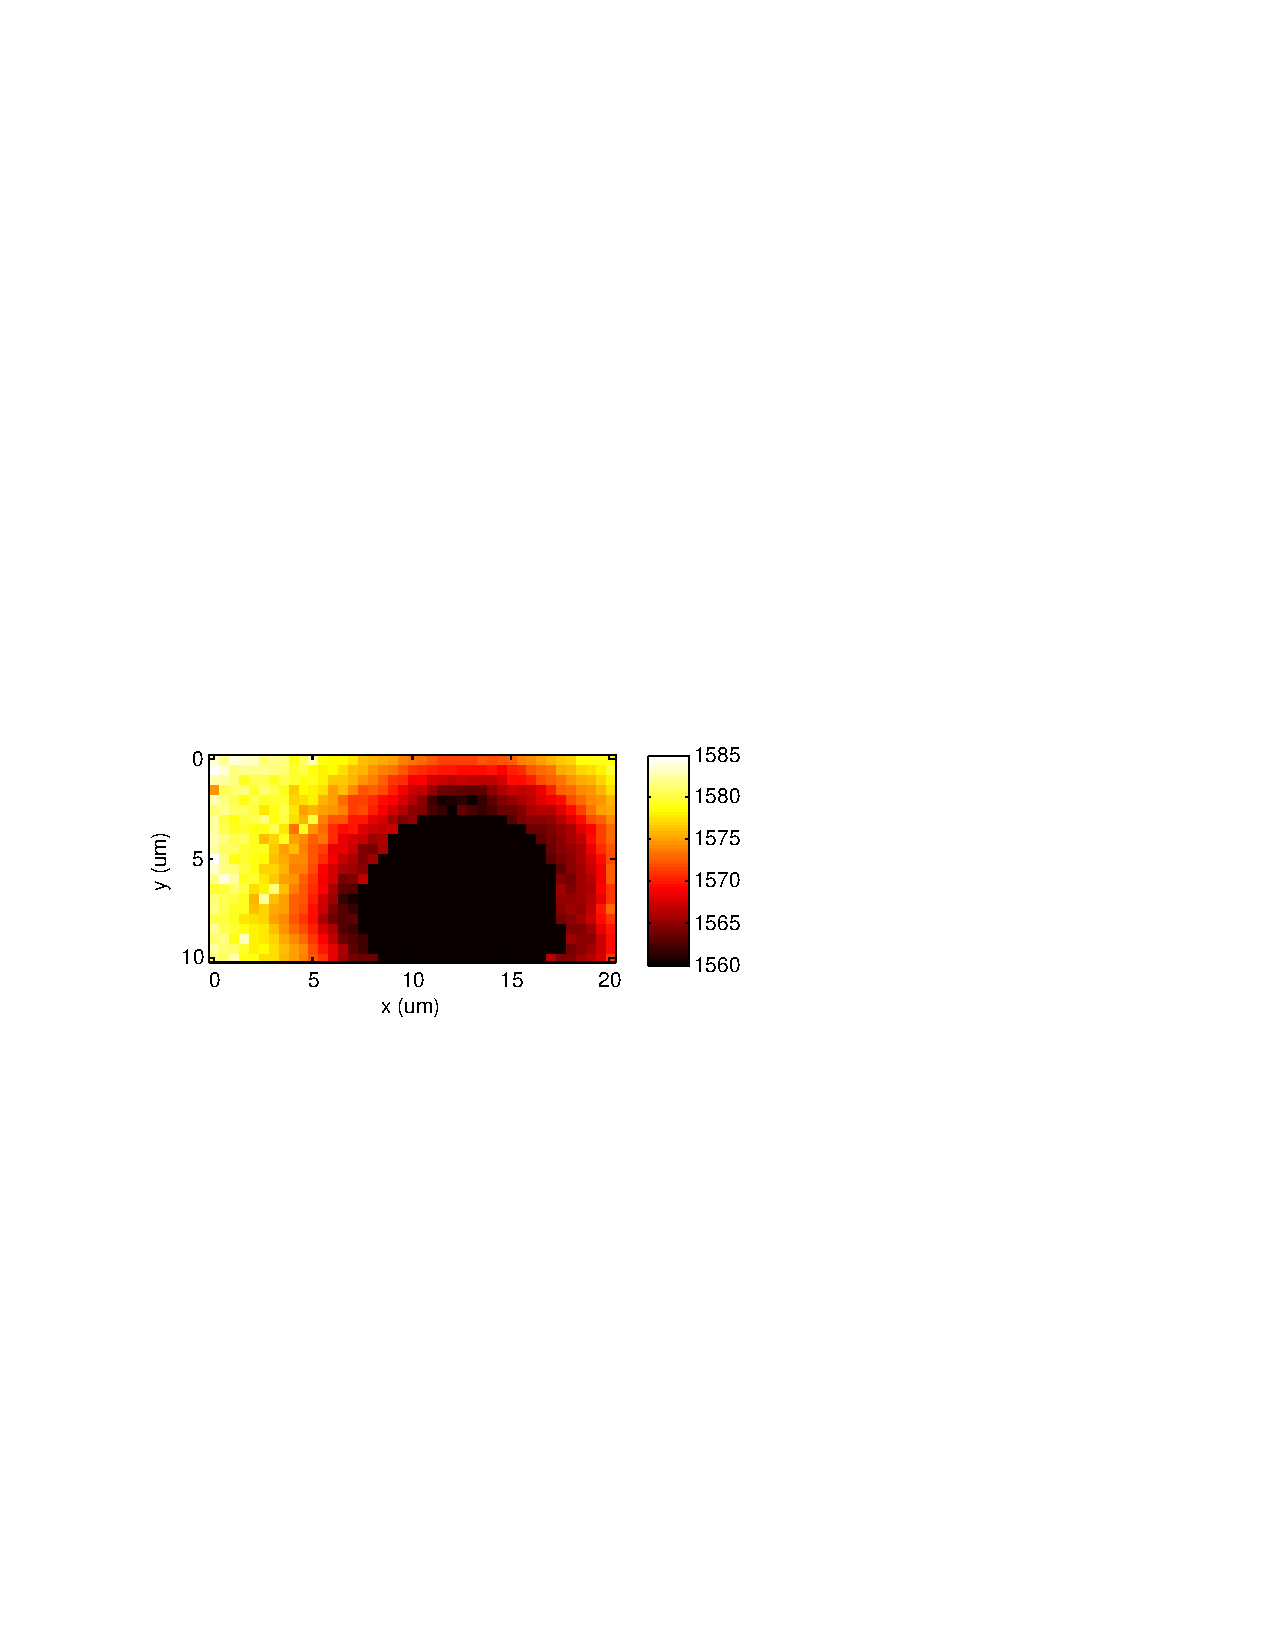
\includegraphics[scale=1]{Figs_Friction/x2.pdf}};
	\node at (-4.75,2.75) {\textbf{b:} $\omega^+$};
	\node at (-.065,-.08) {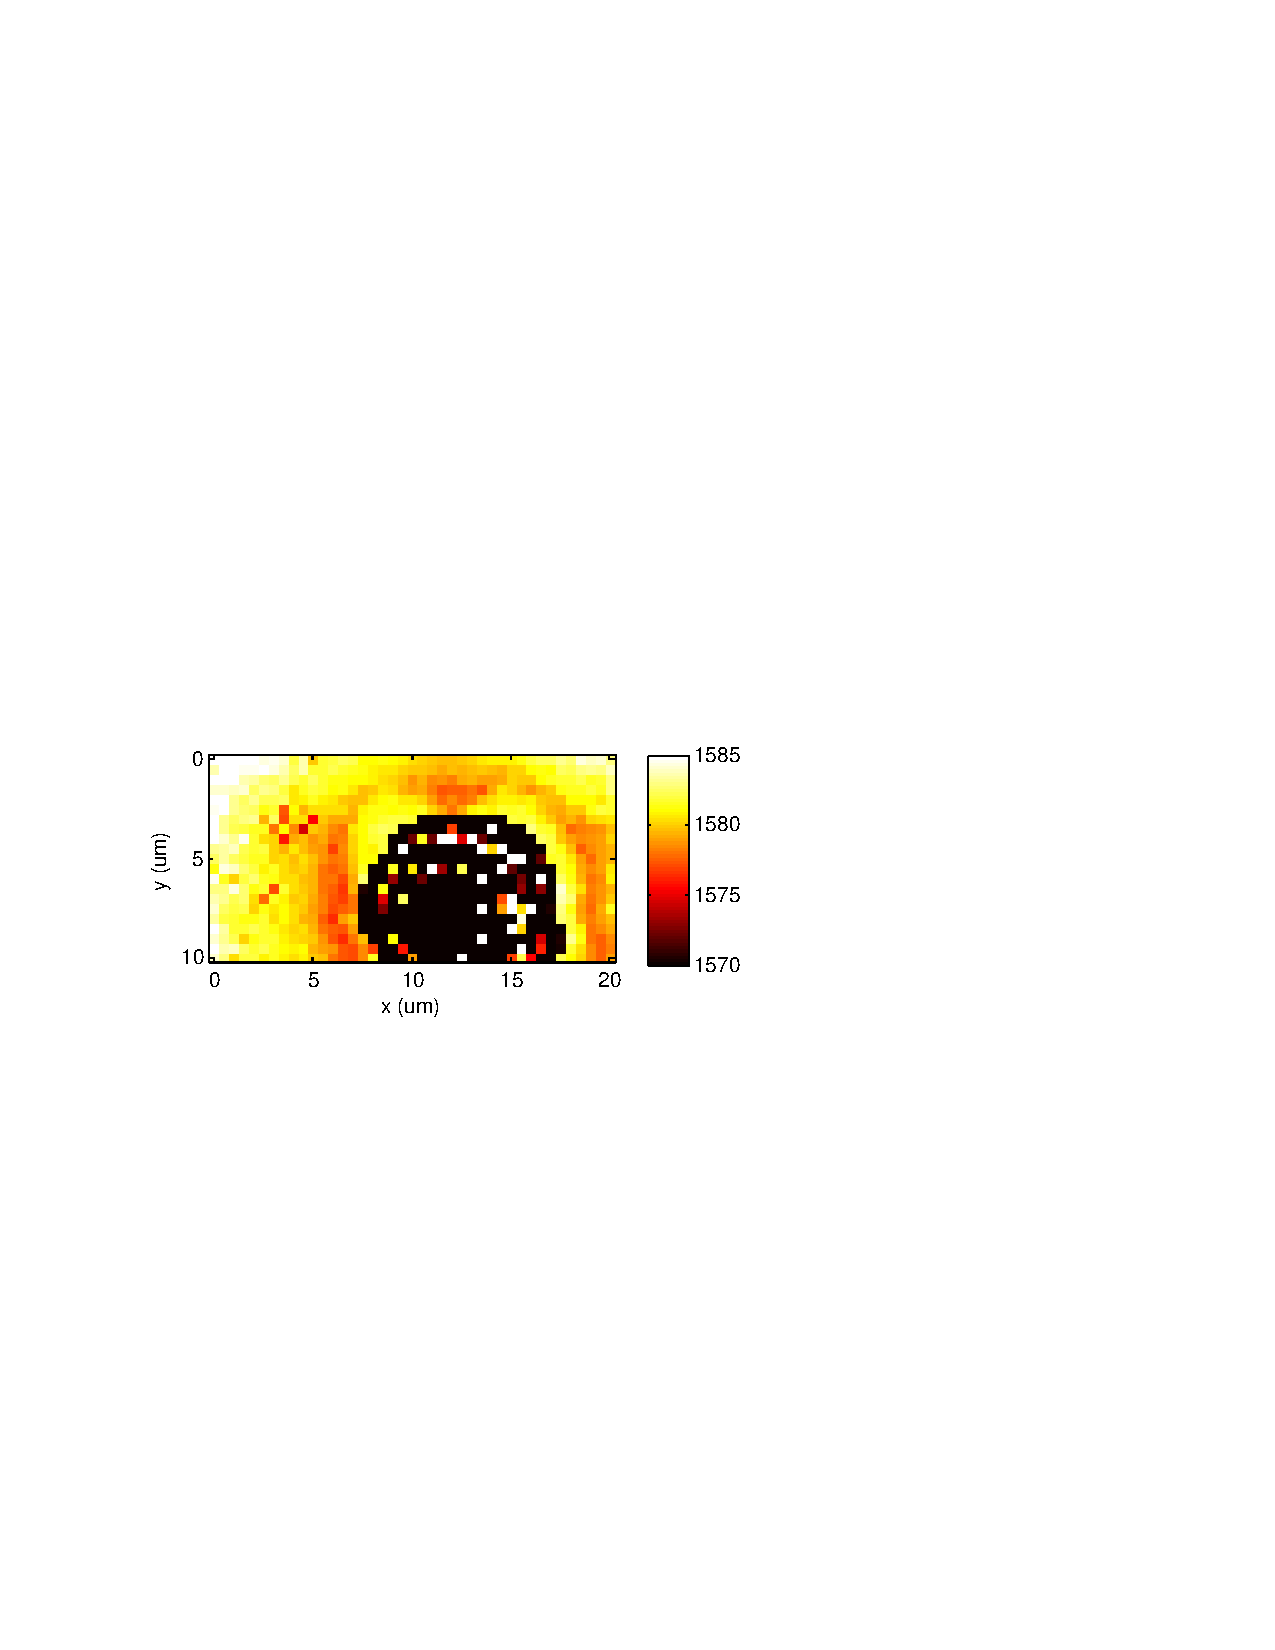
\includegraphics[scale=1]{Figs_Friction/x3.pdf}};
\end{tikzpicture}